\documentclass[../main.tex]{subfiles}
%\usepackage{algorithm}
%\usepackage{algorithmic}


\everymath{\displaystyle}
\def\arraystretch{2.0}
\begin{document}
\setlength{\delimitershortfall}{0pt}

\chapter{Verification}\label{sec:verification}
\addcontentsline{lof}{chapter}{Verification}
\minitoc
%\sectlof
%\sectlot

After chapter~\ref{sec:fluid_mechanics} described the basic equations of fluid mechanics, discretization of this equations with \ac{FV} and \ac{FE} schemes in chapter~\ref{sec:finite_volume_method}, and an introduction to \ac{SA}, the expressions for the actual derivatives have been derived in chapter~\ref{sec:SA}. This has been done for both the body-fitted and the embedded~\ref{sec:embedded_boundary_method} framework of AERO-F.\\
This chapter is denoted to a thorough validation of the obtained derivatives. As described in \ref{sec:SA}, AERO-F handles both sensitivities with respect to far-field variables(e.g. angle of attack) as well as shape sensitivities. Both types require to be handled fundamentally different. While the first type leads to derivatives mainly in the far field boundary conditions, the latter one interferes with the wall treatment. More importantly, as shown in chapters~\ref{sec:fluid_jacobian} and \ref{sec:dresidual_by_absvar}, in the embedded case, doing shape sensitivities leads to additional derivatives with regards to the intersector.\\
For all those reasons, the verification provided in this chapter deals with both $\machnum_{\infty}$-sensitivity as well as shape-sensitivity. More over we will provide plots for both the body-fitted and the embedded case.

\section{Approach}\label{sec:verification_approach}
The question of how to verify the obtained sensitivities is anything but straightforward.\\
The first question is: What can be verified anyway?\\
If we have a look at equation \eqref{eq:full_sa_nostruct}, one can see, that there are two main derivatives: $\pdfrac{\dresidual}{\dfstate}$ and $\pdfrac{\dresidual}{\absvar}$. The derivative with respect to the mesh position $\pdfrac{\dresidual}{\dmpos}$ is not validated here, since it is obtained from SDESIGN and taken for granted.\\
The basic idea that we exploit for verification is to compute a reference solution for the sensitivities by a \ac{FD} of two steady-state simulations. The advantage is, that the sensitivity-module does not have to be used at all to obtain those references, thus it is ensured that potential bugs are not carried over.\\
However, for both of the above quantities, computing a finite difference solution is cumbersome. For the Jacobian $\pdfrac{\dresidual}{\dfstate}$ a simple forward difference would look as follows:
\begin{align}
\pdfrac{\dresidual_i}{\dfstate_j}\bigg\rvert_{\fstate_0}=\frac{\dresidual_i(\dfstate_0+\epsilon\vec{e}_j)-\dresidual_i(\dfstate_0-\epsilon\vec{e}_j)}{2\epsilon}
\end{align}
which would entail an $\order{N}$ number of residual evaluations.\\
As far as $\pdfrac{\dresidual}{\absvar}$ goes, a \ac{FD} verification would be feasible:
\begin{align}
\pdfrac{\dresidual_i}{\machnum_{\infty}}&=\frac{\dresidual(\dfstate_i^{+})-\dresidual(\dfstate_i^{-})}{2\epsilon} \nonumber \\
\dfstate_i^{\pm} &=
\begin{cases}
\dfstate_i\big\rvert_{0}\text{   for internal nodes}\\
\dfstate_i\big\rvert_{\fstate_i(\machnum_i=\machnum_0+\epsilon)}\text{   for boundary nodes}
\end{cases}
\end{align}
which could be done cheaply, and is in fact done in AERO-F if the parameter \texttt{SensitivityAnalysis.SensitivityComputation} is set to \texttt{FiniteDifference}. However, it requires the fluid-state to be updated according to the Mach-number change at the fluid boundary and thus introduces a potential for bugs.\\
Instead, the first quantity to be validated in this thesis is the solution of the linear system described in equation \eqref{eq:full_sa_nostruct}: $\pdfrac{\dfstate}{\absvar}$.\\
this can be done easily by performing a simple \ac{FD} on the solution of two steady-state simulations;
\begin{align}
\tfrac{\dfstate}{\absvar}=\frac{\dfstate(\absvar+\epsilon)-\dfstate(\absvar-\epsilon)}{2 \epsilon}
\end{align}
which involves no extra coding and can be done with a standard steady state solver.
The validation of $\tfrac{\dfstate}{\absvar}$ is provided in figures [\ref{fig:verification_dwdma_ale_Euler},\ref{fig:verification_dwdma_ale_Laminar},\ref{fig:verification_dwdma_ale_RANS}] for the body fitted framework and figures~[\ref{fig:verification_dwdma_emb_Euler},\ref{fig:verification_dwdma_emb_Laminar},\ref{fig:verification_dwdma_emb_RANS}] for the embedded.

Additionally, since the optimization will run on lift and drag, we also validate them with steady state results.
\begin{align}
\tfrac{\optcrit}{\absvar}=\frac{\optcrit(\absvar+\epsilon)-\optcrit(\absvar-\epsilon)}{2 \epsilon}
\end{align}
The validation of integrated forces is provided in figures~[\ref{fig:dLdMa_Euler_ale},\ref{fig:dLdMa_Laminar_ale},\ref{fig:dLdMa_RANS_ale}] for body-fitted computations and in figures~[\ref{fig:dLdMa_Euler_emb},\ref{fig:dLdMa_Laminar_emb},\ref{fig:dLdMa_RANS_emb}] for embedded.



\begin{figure}
\centering
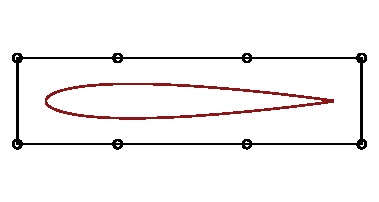
\includegraphics[scale=1.0]{\mainpath/fig/pdf/verificationsetup.pdf}
\caption[Verification setup]{Setup used for the sensitivity verification. A simple NACA0012 profile is considered. The design element concept, as described in section \ref{sec:design_model} is applied. The profile is deformed using a cubic polynomial in x-direction and a linear polynomial in y-direction.}
\label{fig:verification_setup}
\end{figure}

\section{Verification of $\pdfrac{\dfstate}{\absvar}$}\label{sec:verification_dwds}
As explained the first quantity we can reasonably verify is the partial derivative of the fluid state vector $\dfstate$ with respect to the abstract variable. We do this for both a global quantity( free stream mach number $\machnum$) in section \ref{sec:verification_dwds_mach} as well as a shape variable in section~\ref{sec:verification_dwds_shape}
\subsection{Mach-sensitivity}\label{sec:verification_dwds_mach}
For the body-fitted case, the verification of $\tfrac{\dfstate}{\machnum_{\infty}}$ is provided in figure~\ref{fig:verification_dwdma_ale_Euler} for Euler equations, figure~\ref{fig:verification_dwdma_ale_Laminar} for full \ac{NSE} and in figure~\ref{fig:verification_dwdma_ale_RANS} for \ac{NSE} with an additional Spallart-Almares turbulence model.
Additionally, a side by side comparison of the analytic results between all three equation types is also provided in figure~\ref{fig:verification_dwdma_ale_comparison} in order to ensure, that the additional viscous and turbulent terms actually account for a visible difference.\\
For the embedded case, we provide the verification of $\tfrac{\dfstate}{\machnum_{\infty}}$  in figure~\ref{fig:verification_dwdma_emb_Euler} for Euler equation, figure~\ref{fig:verification_dwdma_emb_Laminar} for full \ac{NSE} and in figure~\ref{fig:verification_dwdma_emb_RANS} for \ac{NSE} equations with an additional Spallart-Almares turbulence model.
Again, a side by side comparison of the analytic results between all three equation types is also provided in figure~\ref{fig:verification_dwdma_emb_comparison} in order to ensure that the additional viscous and turbulent terms actually account for a visible difference.


%--------------------------------------------------------------------------------------------
%\section{Body-fitted}
\foreach \vertype in {Euler,Laminar,RANS}{
	%\subsection{Verification $\tfrac{\dfstate}{\machnum_{\infty}}$ for \vertype equations and a body-fitted framework}
	\begin{figure}[t!]
	    \centering
	    \textbf{Verification $\tfrac{\dfstate}{\machnum_{\infty}}$ for {\vertype} equations and a body-fitted framework}\par\medskip    
	    \foreach \n in {1,2,3,5}{
	      \foreach \type in {FD,ana}{
			    \begin{subfigure}[t]{0.4\textwidth}
			        \centering
			        \setlength{\fboxsep}{\valfboxsep}%\valfboxsep=0pt
              \setlength{\fboxrule}{\valfboxrule}%\valfboxrule=1pt
			        \fbox{\includegraphics[width=\linewidth]{\mainpath/fig/studies/StateVector_verification/machsens/ALE/\vertype_component\n_\type}}
			        \caption{$\linepdfrac{\d{w}_\n^{\type}}{\machnum_{\infty}}$}
			    \end{subfigure}%
			    ~ 
	      }~
	      \begin{subfigure}[t]{0.1\textwidth}
	        
\includegraphics[width=0.22\linewidth]{\mainpath/fig/studies/StateVector_verification/colorbar_empty}
	      \end{subfigure}
	      
	    }
	    \caption[Verification $\tfrac{\dfstate}{\machnum_{\infty}}$ {\vertype} equations body-fitted]{Verification of $\tfrac{\dfstate}{\machnum_{\infty}}$ for {\vertype} equations in the body-fitted framework. The \ac{FD} reference solution as described in chapter~\ref{sec:verification_approach} is provided in the left column, the newly implemented analytic derivatives are visualized in the right column. \ac{FD} and analytic solution are plotted using the same color-scheme.}
	    \label{fig:verification_dwdma_ale_\vertype}
	    
	    
	\end{figure}
}

%--------------------------------------------------------------------------------------------
%\section{Embedded}
\foreach \vertype in {Euler,Laminar,RANS}{
	%\subsection{Verification of the \vertype derivatives}
	\begin{figure}[t!]
	    \centering
	    \textbf{Verification of $\tfrac{\dfstate}{\machnum_{\infty}}$ for {\vertype} equations and a embedded framework}\par\medskip    
	    \foreach \n in {1,2,3,5}{
	      \foreach \type in {FD,ana}{
			    \begin{subfigure}[t]{0.4\textwidth}
			        \centering
			        \setlength{\fboxsep}{\valfboxsep}%\valfboxsep=0pt
              \setlength{\fboxrule}{\valfboxrule}%\valfboxrule=1pt
			        \fbox{\includegraphics[width=\linewidth]{\mainpath/fig/studies/StateVector_verification/machsens/Emb/\vertype_component\n_\type}}
			        \caption{$\linepdfrac{\d{w}_\n^{\type}}{\machnum_{\infty}}$}
			    \end{subfigure}%
			    ~ 
	      }~
	      \begin{subfigure}[t]{0.1\textwidth}
	        
\includegraphics[width=0.22\linewidth]{\mainpath/fig/studies/StateVector_verification/colorbar_empty}
	      \end{subfigure}
	      
	    }
	    \caption[Verification of $\tfrac{\dfstate}{\machnum_{\infty}}$ for {\vertype} equations, embedded]{Verification of $\tfrac{\dfstate}{\machnum_{\infty}}$ for {\vertype} equations in the embedded framework. The \ac{FD} reference solution as described in chapter~\ref{sec:verification_approach} is provided in the left column, the newly implemented analytic derivatives are visualized in the right column. \ac{FD} and analytic solution are plotted using the same color-scheme.}
	    \label{fig:verification_dwdma_emb_\vertype}
	    
	\end{figure}
}





%--------------------------------------------------------------------------------------------
%\subsection{Comparison}

%\begin{figure}[t!]
%    \centering
%    \textbf{Comparison of $\tfrac{\dfstate}{\machnum_{\infty}}$ in the body-fitted framework for all 3 equation types}\par\medskip    
%    \foreach \n in {1,2,3,5}{
%      \foreach \simtype in {Euler,Laminar,RANS}{
%		    \begin{subfigure}[t]{0.3\textwidth}
%		        \centering
%			        \setlength{\fboxsep}{\valfboxsep}%\valfboxsep=0pt
%              \setlength{\fboxrule}{\valfboxrule}%\valfboxrule=1pt
%		        \fbox{\includegraphics[width=\linewidth]{\mainpath/fig/studies/StateVector_verification/machsens/ALE/comparison_\simtype_component\n_ana}}
%		        \caption{$\linepdfrac{\d{w_\n^{\simtype}}}{\machnum_{\infty}}$}
%		    \end{subfigure}%
%		    ~ 
%      }~
%	    \begin{subfigure}[t]{0.1\textwidth}
%	      
\includegraphics[width=0.19\linewidth]{\mainpath/fig/studies/StateVector_verification/colorbar_empty}
%	    \end{subfigure}
%      
%    }
%    \caption[Comparison of analytic $\tfrac{\dfstate}{\machnum_{\infty}}$ for all equation types body-fitted]{Comparison of analytic $\tfrac{\dfstate}{\machnum_{\infty}}$ for Euler equations(left column), laminar \ac{NSE} equations (center column) and \ac{NSE} equations with turbulence models (right column) in the body-fitted framework.}
%    \label{fig:verification_dwdma_ale_comparison}
%\end{figure}
%
%
%\begin{figure}[t!]
%    \centering
%    \textbf{Comparison of $\tfrac{\dfstate}{\machnum_{\infty}}$ in the embedded framework for all 3 equation types}\par\medskip    
%    \foreach \n in {1,2,3,5}{
%      \foreach \simtype in {Euler,Laminar,RANS}{
%		    \begin{subfigure}[t]{0.3\textwidth}
%		        \centering
%			        \setlength{\fboxsep}{\valfboxsep}%\valfboxsep=0pt
%              \setlength{\fboxrule}{\valfboxrule}%\valfboxrule=1pt
%		        \fbox{\includegraphics[width=\linewidth]{\mainpath/fig/studies/StateVector_verification/machsens/Emb/comparison_\simtype_component\n_ana}}
%		        \caption{$\linepdfrac{\d{w_\n^{\simtype}}}{\machnum_{\infty}}$}
%		    \end{subfigure}%
%		    ~ 
%      }~
%	    \begin{subfigure}[t]{0.1\textwidth}
%	      
\includegraphics[width=0.19\linewidth]{\mainpath/fig/studies/StateVector_verification/colorbar_empty}
%	    \end{subfigure}
%      
%    }
%    \caption[Comparison of analytic $\tfrac{\dfstate}{\machnum_{\infty}}$ for all equation types embedded]{Comparison of analytic $\tfrac{\dfstate}{\machnum_{\infty}}$ for Euler equations(left column), laminar \ac{NSE} equations (center column) and \ac{NSE} equations with turbulence models (right column) in the embedded framework.}
%    \label{fig:verification_dwdma_emb_comparison}
%\end{figure}



\FloatBarrier

%--------------------------------------------------------------------------------------------
%--------------------------------------------------------------------------------------------


\subsection{Shape-sensitivity}\label{sec:verification_dwds_shape}
The verification of $\tfrac{\dfstate}{\absvar}$ for body-fitted simulations is provided in figure~\ref{fig:verification_dwds_ale_Euler} for Euler equation, figure~\ref{fig:verification_dwds_ale_Laminar} for full \ac{NSE} and in figure~\ref{fig:verification_dwds_ale_RANS} for \ac{NSE} with an additional Spallart-Almares turbulence model.
Additionally, a side by side comparison of the analytic results between all three equation types is also provided in figure~\ref{fig:verification_dwds_ale_comparison} in order to ensure that the additional viscous and turbulent terms actually account for a visible difference.
\\
For the embedded case, we provide the verification of $\tfrac{\dfstate}{\absvar}$  in figure~\ref{fig:verification_dwds_emb_Euler} for Euler equation, figure~\ref{fig:verification_dwds_emb_Laminar} for full \ac{NSE} and in figure~\ref{fig:verification_dwds_emb_RANS} for \ac{NSE} with an additional Spallart-Almares turbulence model.
Again, a side by side comparison of the analytic results between all three equation types is also provided in figure~\ref{fig:verification_dwds_emb_comparison} in order to ensure that the additional viscous and turbulent terms actually account for a visible difference.
%--------------------------------------------------------------------------------------------
%\section{Body-fitted}
\foreach \vertype in {Euler,Laminar,RANS}{
	%\subsection{Verification of the \vertype derivatives}
	\begin{figure}[t!]
	    \centering
	    \textbf{Verification $\tfrac{\dfstate}{\absvar}$ for {\vertype} equations and a body-fitted framework}\par\medskip    
	    \foreach \n in {1,2,3,5}{
	      \foreach \type in {FD,ana}{
			    \begin{subfigure}[t]{0.4\textwidth}
			        \centering
			        \setlength{\fboxsep}{\valfboxsep}%\valfboxsep=0pt
              \setlength{\fboxrule}{\valfboxrule}%\valfboxrule=1pt
			        \fbox{\includegraphics[width=\linewidth]{\mainpath/fig/studies/StateVector_verification/shapesens/ALE/\vertype_component\n_\type}}
			        \caption{$\linepdfrac{\d{w}_\n^{\type}}{\absvar}$}
			    \end{subfigure}%
			    ~ 
	      }~
	      \begin{subfigure}[t]{0.1\textwidth}
	        
\includegraphics[width=0.22\linewidth]{\mainpath/fig/studies/StateVector_verification/colorbar_empty}
	      \end{subfigure}
	      
	    }
	    \caption[Verification of $\tfrac{\dfstate}{\absvar}$ {\vertype} for equations, body-fitted]{Verification of $\tfrac{\dfstate}{\absvar}$ for {\vertype} equations in the body-fitted framework.
	    The \ac{FD} reference solution as described in chapter~\ref{sec:verification_approach} is provided in the left column, the newly implemented analytic derivatives are visualized in the right column. \ac{FD} and analytic solution are plotted using the same color-scheme.}
	    \label{fig:verification_dwds_ale_\vertype}
	    
	\end{figure}
}

%--------------------------------------------------------------------------------------------
%\section{Embededd}

\foreach \vertype in {Euler,Laminar,RANS}{
	%\subsection{Verification of the \vertype derivatives}
	\begin{figure}[t!]
	    \centering
	    \textbf{Verification $\tfrac{\dfstate}{\absvar}$ for {\vertype} equations and a embedded framework}\par\medskip    
	    \foreach \n in {1,2,3,5}{
	      \foreach \type in {FD,ana}{
			    \begin{subfigure}[t]{0.4\textwidth}
			        \centering
			        \setlength{\fboxsep}{\valfboxsep}%\valfboxsep=0pt
              \setlength{\fboxrule}{\valfboxrule}%\valfboxrule=1pt
			        \fbox{\includegraphics[width=\linewidth]{\mainpath/fig/studies/StateVector_verification/shapesens/Emb/\vertype_component\n_\type}}
			        \caption{$\linepdfrac{\d{w}_\n^{\type}}{\absvar}$}
			    \end{subfigure}%
			    ~ 
	      }~
	      \begin{subfigure}[t]{0.1\textwidth}
	        
\includegraphics[width=0.22\linewidth]{\mainpath/fig/studies/StateVector_verification/colorbar_empty}
	      \end{subfigure}
	      
	    }
	    \caption[Verification $\tfrac{\dfstate}{\absvar}$ {\vertype} equations embedded]{Verification of $\tfrac{\dfstate}{\absvar}$ for {\vertype} equations in the embedded framework.
	    The \ac{FD} reference solution as described in chapter~\ref{sec:verification_approach} is provided in the left column, the newly implemented analytic derivatives are visualized in the right column. \ac{FD} and analytic solution are plotted using the same color-scheme.}
	    \label{fig:verification_dwds_emb_\vertype}
	    
	\end{figure}
}


%--------------------------------------------------------------------------------------------
%\subsection{Comparison}

\begin{figure}[t!]
    \centering
    \textbf{Comparison of $\tfrac{\dfstate}{\absvar}$ in the body-fitted framework for all 3 equation types}\par\medskip    
    \foreach \n in {1,2,3,5}{
      \foreach \simtype in {Euler,Laminar,RANS}{
		    \begin{subfigure}[t]{0.3\textwidth}
		        \centering
			        \setlength{\fboxsep}{\valfboxsep}%\valfboxsep=0pt
              \setlength{\fboxrule}{\valfboxrule}%\valfboxrule=1pt
		        \fbox{\includegraphics[width=\linewidth]{\mainpath/fig/studies/StateVector_verification/shapesens/ALE/\simtype_component\n_ana}}
		        \caption{$\linepdfrac{\d{w_\n^{\simtype}}}{\absvar}$}
		    \end{subfigure}%
		    ~ 
      }~
	    \begin{subfigure}[t]{0.1\textwidth}
	      
\includegraphics[width=0.19\linewidth]{\mainpath/fig/studies/StateVector_verification/colorbar_empty}
	    \end{subfigure}
      
    }
    \caption[Comparison of analytic $\tfrac{\dfstate}{\machnum_{\infty}}$ for all equation types, body-fitted]{Comparison of analytic $\tfrac{\dfstate}{\machnum_{\infty}}$ for Euler equations(left column), laminar \ac{NSE} equations (center column) and \ac{NSE} equations with turbulence models (right column) in the body-fitted framework. The purpose of this comparison is to show that each additional equation term actually has a visible impact on the solution, thus we ensure that the separate verification of each equation type in the previous chapter actually captured all terms.}
    \label{fig:verification_dwds_ale_comparison}
\end{figure}

\begin{figure}[t!]
    \centering
    \textbf{Comparison of $\tfrac{\dfstate}{\absvar}$ in the embedded framework for all 3 equation types}\par\medskip    
    \foreach \n in {1,2,3,5}{
      \foreach \simtype in {Euler,Laminar,RANS}{
		    \begin{subfigure}[t]{0.3\textwidth}
		        \centering
			        \setlength{\fboxsep}{\valfboxsep}%\valfboxsep=0pt
              \setlength{\fboxrule}{\valfboxrule}%\valfboxrule=1pt
		        \fbox{\includegraphics[width=\linewidth]{\mainpath/fig/studies/StateVector_verification/shapesens/Emb/\simtype_component\n_ana}}
		        \caption{$\linepdfrac{\d{w_\n^{\simtype}}}{\absvar}$}
		    \end{subfigure}%
		    ~ 
      }~
	    \begin{subfigure}[t]{0.1\textwidth}
	      
\includegraphics[width=0.19\linewidth]{\mainpath/fig/studies/StateVector_verification/colorbar_empty}
	    \end{subfigure}
      
    }
    \caption[Comparison of analytic $\tfrac{\dfstate}{\machnum_{\infty}}$ for all equation types, embedded]{Comparison of analytic $\tfrac{\dfstate}{\machnum_{\infty}}$ for Euler equations(left column), laminar \ac{NSE} equations (center column) and \ac{NSE} equations with turbulence models (right column) in the embedded framework. The purpose of this comparison is to show that each additional equation term actually has a visible impact on the solution, thus we ensure that the separate verification of each equation type in the previous chapter actually captured all terms. }
    \label{fig:verification_dwds_emb_comparison}
\end{figure}






\end{document}





